\chapter{Justificaci�n} 

La compa��a McKinsey\rq s public� un estudio en Octubre de 2013 \cite{mckinsey}  en el que valora el potencial de los Datos Abiertos en t�rminos econ�micos de siete sectores de actividad: educaci�n, transporte, productos de consumo, energ�a el�ctrica, petr�leo, gas, salud y econom�a familiar. \\ 

\begin{figure}[h!]
  \centering
    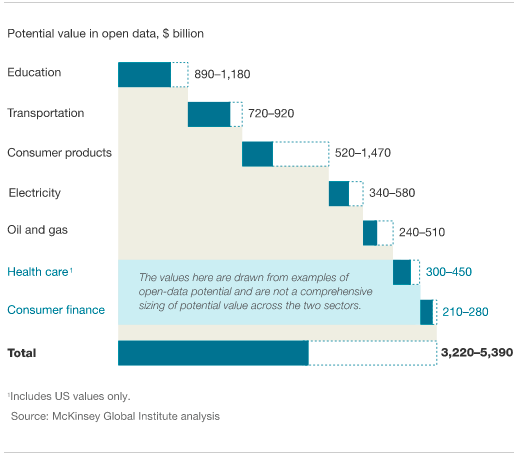
\includegraphics[width=0.8\textwidth]{Images/EstudioMckinsey}
    \caption{ Los datos abiertos pueden ayudar a generar mas de 3 billones de d�lares al a�o en el mundo.}
\end{figure}

La investigaci�n sugiere que esos siete sectores exclusivamente pudieran generar mas de 3 billones de d�lares al a�o de los cuales 1,1 bill�n corresponde a Estados Unidos, 900.000 millones a Europa y los otros 1,7 billones al resto del mundo como resultado de la utilizaci�n de datos abiertos. \\

Otro punto interesante en el estudio, revela c�mo se ha incrementado el n�mero de iniciativas de portales de datos abiertos as� como el n�mero de conjuntos de datos disponibles en cada portal. Por ejemplo, en 2009, el Gobierno de Estados Unidos public� los primeros 47 conjuntos de datos y avanz� r�pidamente hasta llegar a m�s de 90000 en Octubre de 2013.  El Gobierno del Reino Unido alcanza los 10000 conjuntos de datos para esa misma fecha. \\

Por su parte, M�xico se integr� a esta iniciativa en Abril de 2014 y a la fecha en Abril de 2015 cuenta con un total de 358 conjuntos de datos.\\

Estad�sticas como la anterior est� dando pie para la creaci�n de nuevos negocios y ayudando a compa��as ya establecidas a explorar nuevos segmentos de mercado, definir nuevos productos y servicios y mejorar la eficiencia y efectividad de sus operaciones.\\

A�n cuando el fen�meno de datos abiertos a�n esta en sus inicios en nuestro pa�s, podemos observar un claro potencial para utilizar la informaci�n como un instrumento para ayudar a las instituciones gubernamentales a reemplazar la toma de decisiones tradicional por un enfoque orientado a datos. El an�lisis de datos abiertos tambi�n puede ayudar a descubrir preferencias de los ciudadanos, permitiendo a las instituciones mejorar sus servicios y descubrir anomal�as y problemas. \\

Con base en esta informaci�n es que desarrollar una aplicaci�n enfocada a facilitar el proceso de b�squeda y an�lisis de los datos abiertos disponibles prueba ser de gran conveniencia y viabilidad en nuestro entorno global actual.\\